\documentclass{article}

%\usepackage{fancyhdr}
%\usepackage{extramarks}
\usepackage{amsmath}
%\usepackage{amsthm}
\usepackage{amsfonts}
%\usepackage{tikz}
%\usepackage{enumerate}
\usepackage{graphicx}
\graphicspath{ {Images/} }
%\usepackage[plain]{algorithm}
%\usepackage{algpseudocode}
%\usepackage[document]{ragged2e}
%\usepackage{textcomp}

%\usetikzlibrary{automata,positioning}

%
% Basic Document Settings
%

%\topmargin=-0.45in
%\evensidemargin=0in
%\oddsidemargin=0in
%\textwidth=6.5in
%\textheight=9.0in
%\headsep=0.25in

\linespread{1.1}
\setlength{\parskip}{1em}

%\pagestyle{fancy}
%\lhead{\hmwkAuthorName}
%\chead{\hmwkClass\ (\hmwkClassInstructor): \hmwkTitle}
%\rhead{\firstxmark}
%\lfoot{\lastxmark}
%\cfoot{\thepage}

%\renewcommand\headrulewidth{0.4pt}
%\renewcommand\footrulewidth{0.4pt}

%\setlength\parindent{0pt}

%
% Create Problem Sections
%

%\newcommand{\enterProblemHeader}[1]{
%    \nobreak\extramarks{}{Question \arabic{#1} continued on next page\ldots}\nobreak{}
%    \nobreak\extramarks{Question \arabic{#1} (cont.)}{Question \arabic{#1} continued on next page\ldots}\nobreak{}
%}
%
%\newcommand{\exitProblemHeader}[1]{
%    \nobreak\extramarks{Question \arabic{#1} (cont.)}{Question \arabic{#1} continued on next page\ldots}\nobreak{}
%    \stepcounter{#1}
%    \nobreak\extramarks{Question \arabic{#1}}{}\nobreak{}
%}
%
%\setcounter{secnumdepth}{0}
%\newcounter{partCounter}
%\newcounter{homeworkProblemCounter}
%\setcounter{homeworkProblemCounter}{1}
%\nobreak\extramarks{Problem \arabic{homeworkProblemCounter}}{}\nobreak{}

%
% Homework Problem Environment
%
% This environment takes an optional argument. When given, it will adjust the
% problem counter. This is useful for when the problems given for your
% assignment aren't sequential. See the last 3 problems of this template for an
% example.
%
%\newenvironment{homeworkProblem}[1][-1]{
%    \ifnum#1>0
%        \setcounter{homeworkProblemCounter}{#1}
%    \fi
%    \section{Problem \arabic{homeworkProblemCounter}}
%    \setcounter{partCounter}{1}
%    \enterProblemHeader{homeworkProblemCounter}
%}{
%    \exitProblemHeader{homeworkProblemCounter}
%}

%
% Homework Details
%   - Title
%   - Due date
%   - Class
%   - Section/Time
%   - Instructor
%   - Author
%

%\newcommand{\hmwkTitle}{Homework 8}
%\newcommand{\hmwkDueDate}{September 14, 2017}
%\newcommand{\hmwkClass}{Stats 100B}
%%\newcommand{\hmwkClassTime}{Section A}
%\newcommand{\hmwkClassInstructor}{N. Christou}
%\newcommand{\hmwkAuthorName}{\textbf{G. Faletto} }

%
% Title Page
%

%\title{
%    \vspace{2in}
%    \textmd{\textbf{Statistics 100B: Introduction to Mathematical Statistics:\ \hmwkTitle}}\\
%    \normalsize\vspace{0.1in}\small{Due\ on\ \hmwkDueDate}\\
%    \vspace{0.1in}\large{\textit{Instructor: Nicolas Christou\ }}
%    \vspace{3in}
%}
%
%\author{Gregory Faletto \\ UID: 105066274}
%\date{}
%
%\renewcommand{\part}[1]{\textbf{\large Part \Alph{partCounter}}\stepcounter{partCounter}\\}

%
% Various Helper Commands
%

% Useful for algorithms
\newcommand{\alg}[1]{\textsc{\bfseries \footnotesize #1}}

% For derivatives
\newcommand{\deriv}[2]{\frac{\mathrm{d} #1}{\mathrm{d} #2}}

% For partial derivatives
\newcommand{\pderiv}[2]{\frac{\partial #1}{\partial #2}}

% Integral dx
\newcommand{\dx}{\mathrm{d}x}

% Alias for the Solution section header
\newcommand{\solution}{\textbf{\large Solution}}

% Probability commands: Expectation, Variance, Covariance, Bias
\newcommand{\E}{\mathrm{E}}
\newcommand{\Var}{\mathrm{Var}}
\newcommand{\Cov}{\mathrm{Cov}}
\newcommand{\Bias}{\mathrm{Bias}}

% Tilde
\newcommand{\textapprox}{\raisebox{0.5ex}{\texttildelow}}

\begin{document}

%\maketitle

%\pagebreak

\begin{centering}
\section*{Live Nation Project Summary}
\end{centering}

\begin{center}
Gregory Faletto \\
gfaletto@wustl.edu
\end{center}

During my internship with Live Nation, I created an algorithm to predict the future concert \textit{set lists} of bands using their database on setlist.fm. A \textit{set list} is an ordered list of the songs a band plays at a particular concert. Setlist.fm contains a database of past concert set lists of each band, including the date and the location of the concert.

The basic idea of my algorithm is that for every song the band has ever played in a concert listed on setlist.fm, a \textit{song score} is created by taking a sum of the number of times that the band played the song at concerts in the setlist.fm database---except the sum is weighted by recency of the concert, so that more recent performances count more and less recent ones are discounted. This approach accounts for the fact that a band's new set lists are more likely to be similar to their most recent concerts, but still exploits all of the data in the database to some degree.

The details of how the algorithm works follow. The band must be specified; each band has an identification number called an \textit{mbid} which can be found on the band's profile page on setlist.fm\footnote{One easy way to locate this is by searching on Google for the band's name and ``setlist.fm," e.g., ``Red Hot Chili Peppers setlist.fm."}. The user specifies the identification number in the header of the R script I wrote. Some other parameters which will be described later are also specified in the header.

Next the script can be run in R. The script makes a call to the setlist.fm API and downloads JSON files of all of the band's set lists in the database. The script uses the \texttt{jsonLite} R package to parse the data and creates an \(n \times p\) matrix \(\boldsymbol{A}\). Each of the \(n\) songs in the database has its own row in \(\boldsymbol{A}\), and each of the \(p\) columns of \(\boldsymbol{A}\) corresponds to a particular concert, ordered from most to least recent. Matrix element \(A_{ij}\) equals 1 if song \(i\) was played at concert \(j\), and 0 otherwise.

Next a \(p\)-dimensional vector of recency weights \(\boldsymbol{v}\) is created. Let the difference in time between the date the algorithm is run and concert \(j\) be \(\Delta t_j\).  \(\Delta t_j\) is calculated in years (though decimals are allowed) for each concert, and then \(v_j\) is calculated in the following way: \begin{equation}v_j = \bigg(\frac{1}{2} \bigg)^{\Delta t_j/\lambda}\end{equation}where \(\lambda > 0\) is a tuning parameter. Note that as \(\Delta t_j\) increases, \(v_j\) decreases; that is, the longer ago concerts have taken place, the less they will be weighted in the song score. Also note that since \(0 \leq \Delta t_j < \infty\), \(0 < v_j \leq 1\), so weights are always between 0 and 1.

The effect of \(\lambda\) is that for larger values the weights \(\boldsymbol{v}\) are slower to decrease in value (so less recent concerts are less discounted). \(\lambda\) can be thought of as the ``half-life" of weights for concerts; every \(\lambda\) years, the weight is multiplied by another power of \(\frac{1}{2}\). Consider the end behavior of \(v_j\) as a function of \(\lambda\): \begin{equation}\lim_{\lambda \to \infty} v_j = 1 \end{equation}so for very large \(\lambda\), the weights all approximately equal 1 regardless of \(\Delta t_j\), so all concerts are weighted roughly equally regardless of elapsed time.

On the other hand, \begin{equation}\lim_{\lambda \to 0^+} v_j = 0 \text{ if } \Delta t_j > 0 \end{equation} so for very small \(\lambda\), all but the most recent concert have essentially 0 weight.

\(\lambda = 5\) seemed to work fairly well, but this could be fiddled with more.

The total number of times song \(i\) was played at every concert in the database for this band is given by \begin{equation} \sum_{j=1}^p A_{ij} \end{equation}If this sum is weighted by the recency weights \(\boldsymbol{v}\), it yields the song score \(c_i\) for song \(i\): \begin{equation}c_i = \sum_{j=1}^p A_{ij}v_j \end{equation}This computation is done by the algorithm for every song \(i\) simultaneously by computing the product \begin{equation}\boldsymbol{A} \boldsymbol{v} = \boldsymbol{c} \end{equation}where \(\boldsymbol{c}\) is an \(n\)-dimensional vector of song scores.

Lastly, \(\boldsymbol{c}\) is sorted in order of decreasing song score. Then the algorithm returns the names of the first \(\ell\) elements of \(\boldsymbol{c}\), which are the \(\ell\) songs with the highest song scores, where \(\ell\) is arbitrary (at the moment it returns 10 songs). 

%\pagebreak

Examples:

\begin{center}
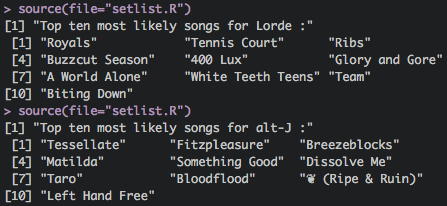
\includegraphics[scale=0.65]{lorde}
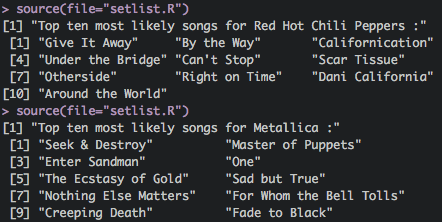
\includegraphics[scale=0.65]{metallica}
\end{center}

\end{document}
